\documentclass{article}
\usepackage{parskip}
\usepackage{graphicx}
\usepackage{geometry}
\usepackage{listings}
\usepackage{xcolor}
\usepackage{hyperref}

 \geometry{
 a4paper,
 total={170mm,257mm},
 left=20mm,
 top=20mm,
 }
 
 
\lstset{language=C++,
                basicstyle=\ttfamily,
                keywordstyle=\color{blue}\ttfamily,
                stringstyle=\color{red}\ttfamily,
                commentstyle=\color{green}\ttfamily,
                morecomment=[l][\color{magenta}]{\#},
                numberstyle=\tiny\color{codegray},
                breakatwhitespace=false,         
    				breaklines=true,                 
    				captionpos=b,                    
    				keepspaces=true,                 
    				numbers=left,                    
    				numbersep=5pt,                  
    				showspaces=false,                
    				showstringspaces=false,
    				showtabs=false,                  
    				tabsize=2
}


\definecolor{codegreen}{rgb}{0,0.6,0}
\definecolor{codegray}{rgb}{0.5,0.5,0.5}
\definecolor{codepurple}{rgb}{0.58,0,0.82}
\definecolor{backcolour}{rgb}{0.95,0.95,0.92}
 
\lstdefinestyle{mystyle}{ 
    commentstyle=\color{codegreen},
    keywordstyle=\color{magenta},
    numberstyle=\tiny\color{codegray},
    stringstyle=\color{codepurple},
    basicstyle=\ttfamily,
    breakatwhitespace=false,         
    breaklines=true,                 
    captionpos=b,                    
    keepspaces=true,                 
    numbers=left,                    
    numbersep=5pt,                  
    showspaces=false,                
    showstringspaces=false,
    showtabs=false,                  
    tabsize=2
}

\title{P\&S SDR: Sat-Tracker Dokumentation}
\date{}
\author{Sean Helle, Charpoan Kong}
\begin{document}

\maketitle

\section*{Ziel}
Das Ziel des Projektes ist einen Satelliten-Tracker zu bauen mit dem Ziel Amateurfunk- und Wettersatelliten zu empfangen u.a auch QSO's dadurch zu führen.

\section*{Systemflow}
Um den Antennenrotor via gPredict zu steuern. Lies ein Pythonscript die Sat. Daten von gPredict via TCP aus und gibt diese per serieller Schnittstelle zum Pico weiter. Der Pico liest den Winkel des Rotors via des Rotorcontrollers aus und steuert die einzelnen Motoren via des Rotorcontrollers. Auch steuert gPredict das Radio und kompensiert die Frequenz zum Satelliten wegen des Dopplereffektes.

\begin{figure}[h]
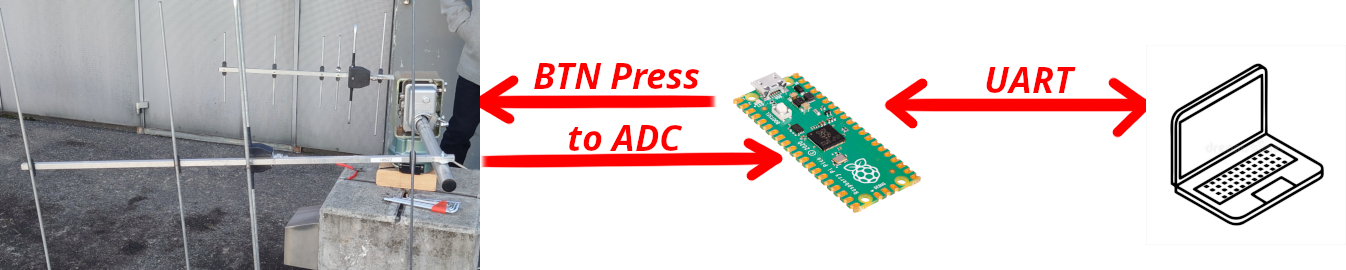
\includegraphics[width=0.5\textwidth]{Over}
\centering 
\caption{Datenflow}
\end{figure}
Der Programflow sieht wie folgt aus:

\begin{figure}[h]
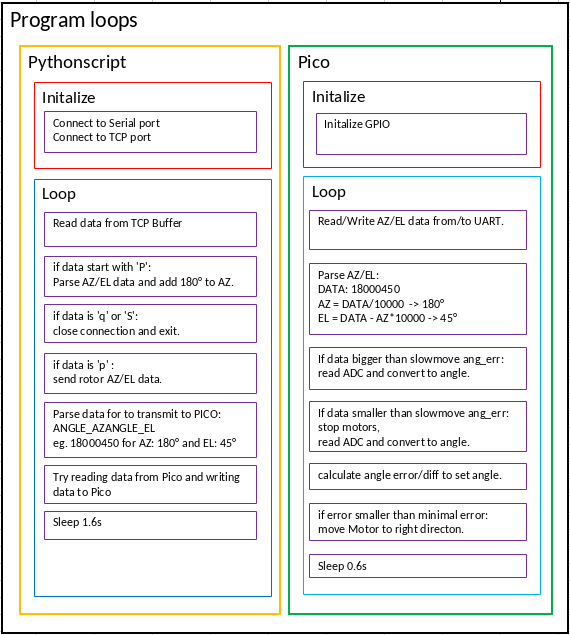
\includegraphics[width=0.5\textwidth]{Flow}
\centering 
\caption{Programmflow}
\end{figure}


\section*{Antennenrotor-Controller}
\subsection*{Picocontroller}
Der Pico steurt den Rotorcontroller durch den DIN-8 Stecker. Durch die \textcolor{blue}{\href{https://dk3wn.info/wp/wp-content/uploads/2018/10/kr5400.pdf}{Dokumentation}} des Controllers wurde herausgegfunden welcher Pin welche Funktion hat. Zudem konnte herausgefunden werden, dass um die einzelnen Motoren anzusteuern, die "Steuer"-Pins auf GND kurzgeschlossen werden müssen.

\begin{figure}[h]
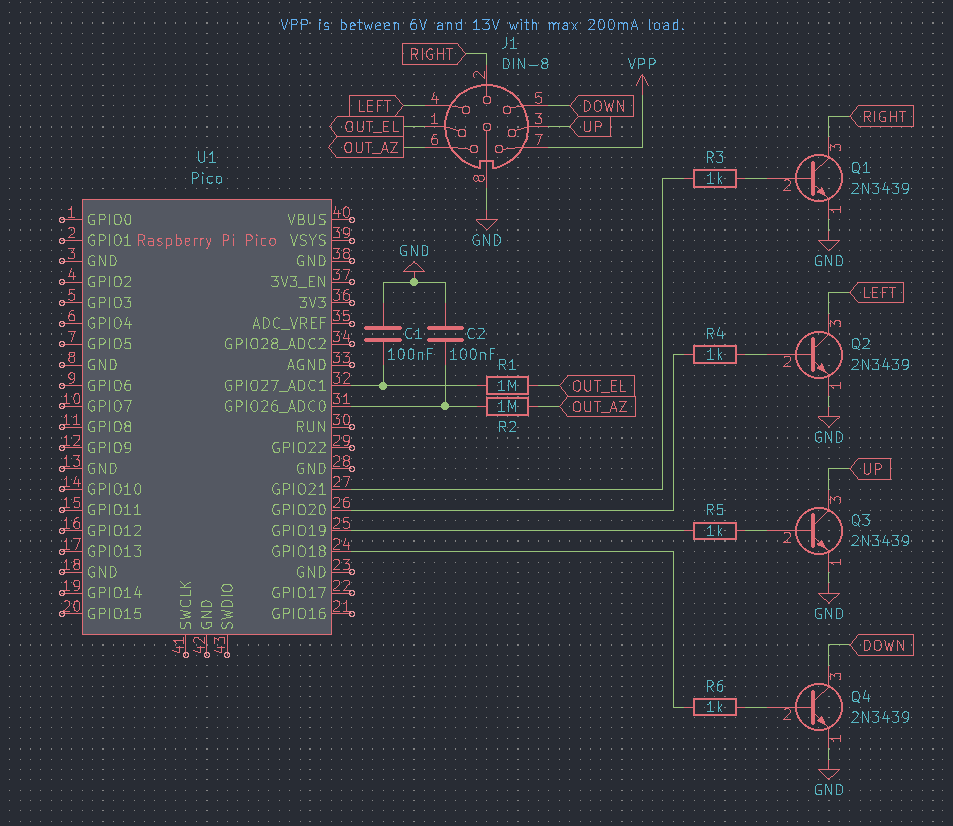
\includegraphics[width=0.5\textwidth]{Wiring}
\centering 
\caption{Schaltplan Pico zu Rotor-Controller}
\end{figure}

\subsection*{Problem mit dem Spannungsabfall}
Durch Anmerkung von Herr Lerjen vom Projekt Stratos, konnte ein Spannungsabfall beobachtet werden, wenn die Motoren stoppen. Dies ist ein Problem, wenn der Motor den Endwinkel erreicht, da die Werte nicht mehr stimmen. Deswegen stoppen alle Motoren beim auslesen der Spannung , wenn der Motor in der nähe des Soll-Winkels ist. Jedoch gab es dann Probleme, da der Motor "oszillierte". Dieses wurde so gelöst, das ein minimaler Abweichungswinkel vom Soll-Winkel eingestellt wurde. Und dass der Motor sich um genug grosse Winkel bewegt.

\section*{Pythonskript}
Gpredict steuert die komerziellen via TCP an und es konnte schon eine Analyse des Protokolls mit Beispiel \textcolor{blue}{\href{https://adventurist.me/posts/0136}{Python-Code}} gefunden werden. Dieser wurde angepasst und der Code zum steuern des Pico wurde hinzugefügt.

\newpage

\section*{Pico code}
\begin{lstlisting}
#include <stdio.h>
#include <math.h>
#include "pico/stdlib.h"
#include "pico/util/queue.h"
#include "pico/multicore.h"
#include "hardware/adc.h"

const uint8_t AZ_R = 21, AZ_L = 20, EL_U = 19, EL_D = 18; //AZ/EL Pins

void MotorControl(){
    uint32_t buffer = 1; //UART buffer

    float azel[2] = {10, 10}; //true AZ/EL angle

    float tgt_azel[2] = {1800,900}; //target AZ/EL angle

    float err_azel[2] = {0, 0}; //error AZ/EL angel
    
    const float minERR = 50; //minimal tolerated error angle: 5deg
    const float slowERR = 100; //error angle when to compensate for voltagedrop: 10deg
    const float maxaz = 3360, maxel = 3520; //max ADC value for max angle -> calibration

    while(true){
        // write data to UART
        printf("%f/%f/%u\n", azel[0], azel[1], buffer);
        fflush(NULL); //flush buffer
        scanf("%u\r\n", &buffer); //read data from UART

        //Parse AZEL
        //Eg. DATA = 18000450
        //AZ = DATA/10000 -> 180 because is integer and everything after the comma is "cut out".
        //EL = DATA - AZ*10000 -> 45
        tgt_azel[0] = (buffer/10000);
        tgt_azel[1] = (buffer - (tgt_azel[0] * 10000));

        //calculate error AZ/EL angle
        err_azel[0] = tgt_azel[0] - azel[0];
        err_azel[1] = tgt_azel[1] - azel[1];

        if(std::abs(err_azel[0]) > slowERR || std::abs(err_azel[1]) > slowERR){ // if error bigger the slowERR -> because of voltage drop
            //read ADC and convert to angle
            adc_select_input(0);
            azel[1] = (((float)adc_read()/maxel)*1800);
            adc_select_input(1);
            azel[0] = ((float)adc_read()/maxaz)*3600;
        }else{ //if smaller than slowERR
            //shutoff all Motors to stop voltage drop
            gpio_put(AZ_R, 0);
            gpio_put(AZ_L, 0);
            gpio_put(EL_U, 0);
            gpio_put(EL_D, 0);

            sleep_ms(400); //wait for motor halt and voltage settling

            //read ADC and convert to error
            adc_select_input(0);
            azel[1] = (((float)adc_read()/maxel)*1800);
            adc_select_input(1);
            azel[0] = ((float)adc_read()/maxaz)*3600;
        }

        //if error is bigger than the minimal error move motors
        if(std::abs(err_azel[0]) > minERR){
            if (err_azel[0] <= 0){
                gpio_put(AZ_R, 0);
                gpio_put(AZ_L, 1);
            }else if(err_azel[0] > 0){
                gpio_put(AZ_R, 1);
                gpio_put(AZ_L, 0);
            }
        }else{
            gpio_put(AZ_R, 0);
            gpio_put(AZ_L, 0);
        }

       if(std::abs(err_azel[1]) > minERR){
            if (err_azel[1] <= 0){
                gpio_put(EL_U, 1);
                gpio_put(EL_D, 0);
            }else if(err_azel[1] > 0){
                gpio_put(EL_U, 0);
                gpio_put(EL_D, 1);
            }
        }else{
            gpio_put(EL_U, 0);
            gpio_put(EL_D, 0);
        }

        sleep_ms(600);//sleep for 0.6s -> enough movement that motor does no oscillate with the error resolution.s
    }
}



int main() {
    //initalize stdlib
    stdio_init_all();
    //initalize adc
    adc_init();

    //initalize ADC_GPIO
    adc_gpio_init(26);
    adc_gpio_init(27);

    //initalize GPIO
    gpio_init(AZ_R);
    gpio_init(AZ_L);
    gpio_init(EL_U);
    gpio_init(EL_D);

    //set GPIO function
    gpio_set_dir(AZ_R, GPIO_OUT);
    gpio_set_dir(AZ_L, GPIO_OUT);
    gpio_set_dir(EL_U, GPIO_OUT);
    gpio_set_dir(EL_D, GPIO_OUT);

    //call MotorControl
    MotorControl();
}

\end{lstlisting}

\newpage
\section*{Python code}
\lstset{style=mystyle, 
		language=Python}
		
\begin{lstlisting}
import socket
import serial
from time import sleep

#initalize Serial port
ser = serial.Serial('/dev/ttyACM2', 9600, timeout=1, parity=serial.PARITY_EVEN)


TCP_IP = '127.0.0.1'
TCP_PORT = 4533
BUFFER_SIZE = 100

#initalize/connect to TCP Port // data parsing form https://adventurist.me/posts/0136
s = socket.socket(socket.AF_INET, socket.SOCK_STREAM)
s.bind((TCP_IP, TCP_PORT))
s.listen(1)

conn, addr = s.accept()
print('Connection address:', addr)

az = 0.0 #AZ from Pico
el = 0.0 #EL from Pico

mmaz = 0 #AZ from gPredict
mmel = 0 #EL from gPredict

maz = '9999' #AZ to Pico
mel = '9999' #EL to Pico

response = " " # data to gPredict
while 1:
	data = conn.recv(BUFFER_SIZE) #read data fronm gPredict
	response = "{}\n{}\n".format(float(f'{az:.2f}'), float(f'{el:.2f}')) #parse data to gPredict

	if (data.startswith(b'P')):
		values = data.split(b' ')
		#print(values)
		mmaz = int(float(values[1])*10)+1800 #convert to integer and add 180deg // 1800 because 0.1deg resolution -> uneccessary...
		mmel = int(float(values[2])*10) #convert to interger

		conn.send(bytes(response, 'utf-8')) #send data from Pico to gPredict
	elif data == b'q\n' or data == b'S\n':
		print("close command, shutting down") #closes Program
		conn.close()
		exit()
	elif data == b'p\n':
		conn.send(bytes(response, 'utf-8')) # send data from Pico to gPredict

	print(response)
	print("moving to az:{} el: {}".format( mmaz, mmel));

	# Parse data for Pico:
	# AZ: 180deg, EL: 45deg -> 18000450

	if(mmaz == 0):
		maz = '000' + str(mmaz)
	if(mmaz < 100):
		maz = '00' + str(mmaz)
	elif(mmaz < 1000):
		maz = '0' + str(mmaz)
	else:
		maz = str(mmaz)

	if(mmel == 0):
		mel = '000' + str(mmel)
	elif(mmel < 100):
		mel = '00' + str(mmel)
	elif(mmel < 1000):
		mel = '0' + str(mmel)
	else:
		mel  = str(mmel)

	#Try to write to the Pico and clear buffer if not print nosend
	try:
		print("az: " + str(mmaz/10) + " el: " + str(mmel/10))
		ser.reset_output_buffer()
		ser.write(bytes(maz + mel +'\r\n', 'ascii'))
		ser.reset_output_buffer()
		
	except:
		print('nosend')
		ser.reset_output_buffer()
		print(str(maz + mel))

	#Try to read to the Pico and clear buffer if not print nor
	try:
		if(ser.in_waiting > 0 ):
			adc = ser.readline()
			ser.reset_input_buffer()
			ser.read_all()
			adc = adc.split(b'/')
			print(adc)
			print("az: " + str(float(adc[0])/10) + " el: " + str(float(adc[1])/10) + " RECEV:" + str(adc[2]))
			az = int(float(adc[0])/10)
			el = int(float(adc[1])/10)
			sleep(0.5)
	except:
		print('nor')

	sleep(1.6) #sleep for clearing buffer.
\end{lstlisting}

\end{document}
